\newcommand{\mcQ}{\mathcal{Q}}
\newcommand{\mcS}{\mathcal{S}}
\newcommand{\mcT}{\mathcal{T}}
\newcommand{\mcD}{\mathcal{D}}
\newcommand{\nwks}[2]{${#1}$-way, ${#2}$-shot}

\chapter{Few-Shot Learning}\label{chap:fsl}
A good machine learning model often requires training with a large number of samples. Humans, on the contrary, learn new concepts and skills much faster and more efficiently. Children who have only seen cats and birds a few times can quickly tell them apart. People who know how to ride a bike are likely to discover how to ride a motorcycle quickly with little or even no demonstration. Is it possible to design a machine learning model with similar properties - can we have it learn new concepts and skills quickly with a few training examples? That is essentially what few-shot learning methods aim to solve.

Despite notable advances in the field of artificial intelligence, two essential aspects of human conceptual intelligence have consistently eluded machine learning and artificial intelligence (AI) systems. 
First, for most interesting kinds of natural and man-made categories of entities, humans can learn a new concept from just one or a few handful examples, whereas many AI models would require several thousands of examples to perform satisfactorily. 
Second, people learn far richer representations than machines do, even for seemingly simple concepts. 
Humans use these representations for a wide variety of tasks such as creating new entities based on the exemplars, classifying objects into parts, grasping relations between concepts, and creating new abstract categories (concepts) by combining existing ideas and concepts. These rich representations also allow us to differentiate between entities.
In stark contrast to this, the best machine learning models and neural networks cannot perform these additional functions using their specialised learnt representations. 
The challenge arises when we wish for AI models to learn new concepts and representations from few examples and ensure that these representations are abstract and flexible.

In this body of work the focus is on few-shot classification of images. Few-shot classification is cast as a task of predicting class labels for a set of unlabelled data points (\textit{query set}) given only a small set of labelled data points (\textit{support set}). Typically, the query and support data points are drawn from the same distribution. 

Few-shot classification methods typically consist of two sequential phases: (i) \textit{pre-training} on a large dataset of \textquote{base} classes, regardless of whether the training is supervised or unsupervised. This is followed by (ii) \textit{fine-tuning} on an unseen dataset consisting of \textquote{novel} classes. Normally, the classes used in the pre-training and fine-tuning are mutually exclusive. In this paper, our focus is on the self-supervised (also sometimes interchangeably called \textquote{unsupervised} in the literature) setting where we have no access to the actual class labels of the \textquote{base} dataset.

To this end, various methods have been proposed and broadly categorised under two different approaches:
\begin{itemize}
    \item \textbf{Meta-learning}. Where an algorithm \textquote{learns how to learn} and aims to find a quickly generalisable model
    \item \textbf{Transfer Learning}. Where the model is trained to learn optimal representations that are generalisable with minimal updates
\end{itemize}

The first approach, \textit{meta-learning}, relies on episodic training that involves creating synthetic \textquote{tasks} to mimic the downstream episodic fine-tuning phase \parencite{Finn2017Model-agnosticNetworks, Hsu2018UnsupervisedMeta-Learning, Khodadadeh2018UnsupervisedClassification, Antoniou2019AssumeAugmentation, Ye2022, lee2021meta, Ji2019UnsupervisedTraining}. 
The second method follows a \textit{transfer learning} approach, where the network trained non-episodically to learn optimal representations in the pre-training phase, which is then followed by an episodic fine-tuning phase \parencite{Medina2020Self-SupervisedClassification, goodemballneed2020, dhillon2019baseline}.
In this method, a feature extractor (encoder) is trained using a form of metric learning to capture the structure of the unlabelled data. 
Next, a simple predictor (conventionally a linear layer) is utilised in conjunction with the pre-trained feature extractor for quick adaptation to the novel classes in the fine-tuning phase.
The better the feature extractor captures the global structure of the unlabelled data, the less the predictor requires training samples and the faster it adapts itself to the unseen classes in the fine-tuning phase (also the testing phase).

We also see a set of supervised approaches that do not rely purely on a convolutional feature extractor. Instead, these approaches also make use of graphs and graph neural networks \parencite{garcia2018fewshot, kim2019edge, yu2022hybrid, yang2020dpgn}. Using a graph neural network (GNN) can help in modelling instance-level and class-level relationships. Graphs can also help propagate labels between labelled and unlabelled samples, this was proposed by \textcite{xiaojin2002learning} and has been applied by \textcite{liu2018learning} in their work. However, it should be noted that graph-based methods have eluded the unsupervised setting.

Several recent studies have questioned the necessity of meta-learning for few-shot classification \parencite{goodemballneed2020, Medina2020Self-SupervisedClassification, dhillon2019baseline, ziko2020laplacian, boudiaf2020information,chen2021self}. They report competitive performance on few-shot benchmarks without episodic training or few-shot task-based experiences during training. These methods follow the second approach and aim to solve the few-shot learning problem by fine-tuning a pre-trained feature extractor with a standard cross-entropy loss.
Some of these methods \parencite{Medina2020Self-SupervisedClassification, goodemballneed2020, das2022confess} in the space demonstrate that the transfer learning approach outperforms meta-learning based methods in standard in-domain and cross-domain settings - where the training and novel classes come from totally different distributions.

\section{Formalising the Few-Shot Learning Problem}\label{sec:formalising-fsl}

In a few-shot setting, the model aims to generalise well and quickly enough on a variety of new and potentially unseen tasks after being trained for optimal performance on various learning tasks.
Each task is associated with a dataset $\mathcal{D}$, containing both inputs and true labels. 
The model parameters of an optimal generalisable model are defined as follows:
\begin{equation}
    \symbfit{\theta}^\star = \arg\min_{\symbfit \theta} \mathbb{E}_{\mathcal{D}\sim \pdata} [\mathcal{L}_{\symbfit \theta}(\mathcal{D})]
\end{equation}

First, we look at how \(\mathcal{D}\) is structured in a standard supervised few-shot setting. 
Consider a labelled dataset of size $M$, $\mathcal{D} = \{({\symbfit x}_i, y_i)\}_{i = 1}^{M}$ of images $\symbfit{x}_i$ and class labels $y_i$. 
This dataset $\mathcal{D}$ is divided into three disjoint subsets: $\left\{\mathcal{D}^\textup{tr}\, \cup\, \mathcal{D}^\textup{val}\, \cup\, \mathcal{D}^\textup{tst}\right\} \in \mathcal{D}$, referring to the training, validation, and test subsets, respectively.
Next, we define a set of randomly sampled tasks $\mathcal{T}_i$ drawn from the training dataset $\mathcal{D}^{\textup{tr}} = \{({\symbfit x}_i, y_i)\}_{i = 1}^{M^\textup{tr}}$ of size $M^\textup{tr}$. A task, $\mathcal{T}_i$, is comprised of two parts: (i) the support set $\mathcal{S}$ from which the model learns, (ii) the query set $\mathcal{Q}$ on which the model is evaluated. The support set $\mathcal{S}=\{\symbfit{x}^{s}_i, y^{s}_i\}_{i=1}^{NK}$ is constructed by drawing $K$ labelled random samples from $N$ different classes, resulting in the so-called ($N$-way, $K$-shot) settings.
The query set $\mathcal{Q}=\{\symbfit{x}^{q}_j\}_{j=1}^{NQ}$ then contains $NQ$ unlabeled samples. By convention, we denote the set $\mathcal{T}_i = \mathcal{S} \cup \mathcal{Q}$ with $(N, K)$.
\begin{figure}[ht]
    \centering
    \captionsetup{justification=centering}
    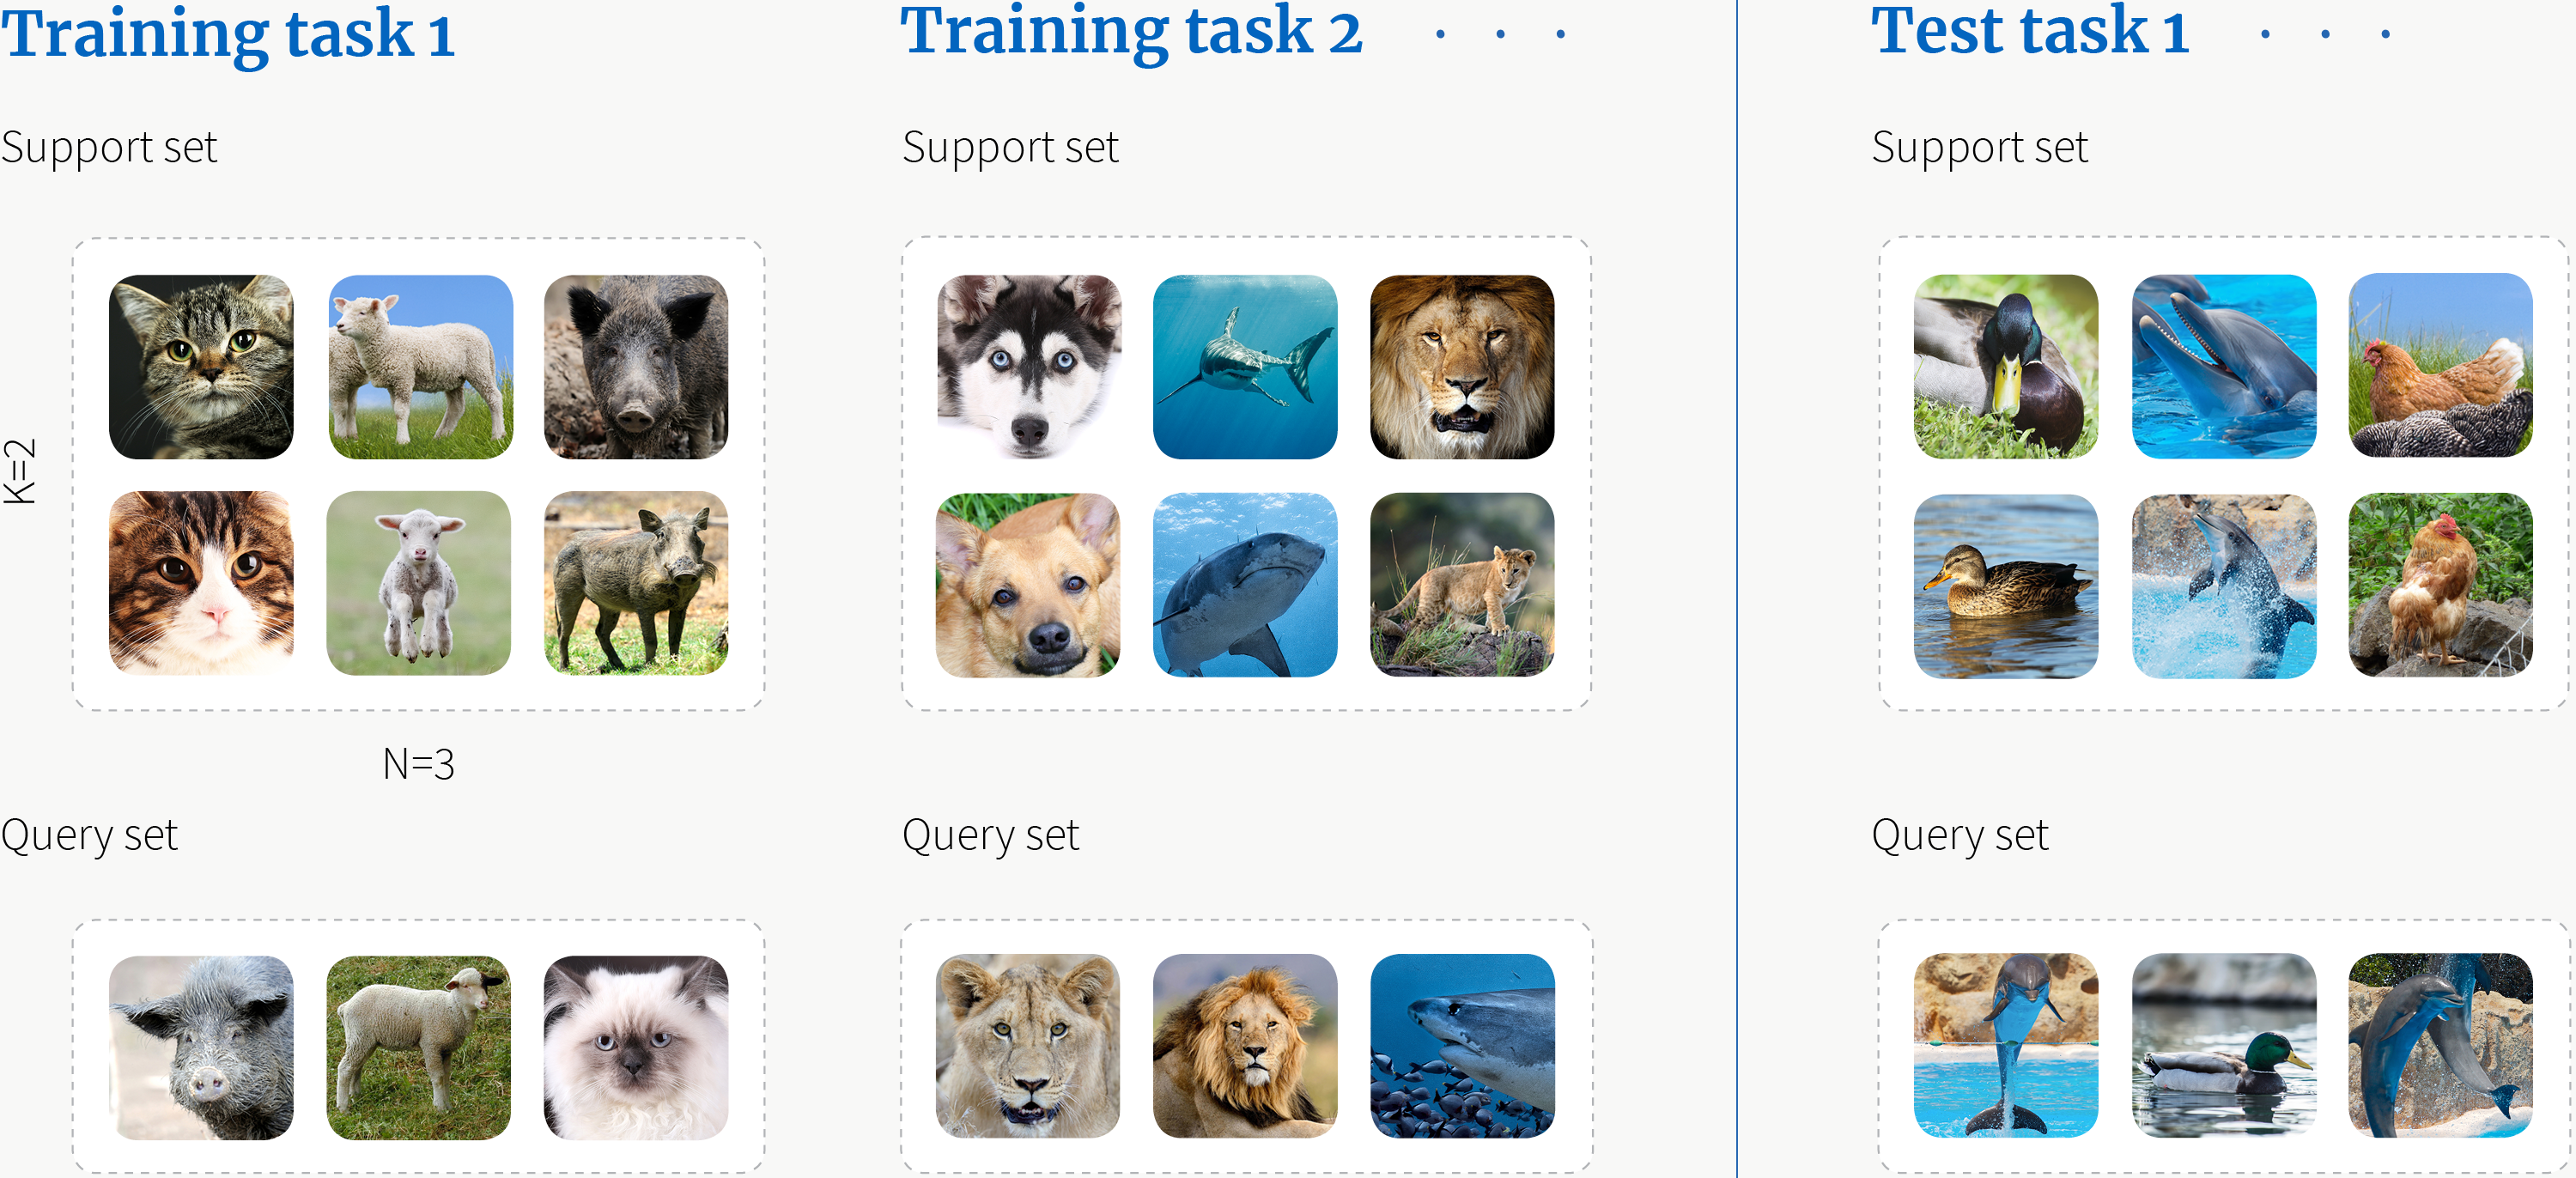
\includegraphics[width=\linewidth]{chapters/assets/fsl/n3k2.png}
    \caption{An example of (\nwks{3}{2}) image classification. Image from Borealis AI\protect\footnotemark}
    \label{fig:fsl-tasks}
\end{figure}
\footnotetext{\url{https://www.borealisai.com/research-blogs/tutorial-2-few-shot-learning-and-meta-learning-i/}}
% In most training routines, tasks are randomly sampled from a task distribution based on the training subset $\mcD_\textup{tr}$ of the dataset $\mcD$ according to the (\nwks{N}{K}) setting, and then the model parameters are updated by back-propagation after each task is processed.This comprises one \textbf{episode}. 
The model is expected to quickly learn the optimal parameters from the $NK$ support data points and apply the learnt weights to classify the $NQ$ unlabelled query data points, on which performance is evaluated.
\Cref{fig:fsl-tasks} shows (\nwks{3}{2}) training tasks, it should be noted that even during testing (downstream classification task) the model is presented with tasks that are in the same (\nwks{3}{2}) form as the training tasks.

\section{Model Agnostic Meta Learning (MAML)}\label{sec:maml}


\begin{wrapfigure}{r}{0.25\linewidth}
    \centering
    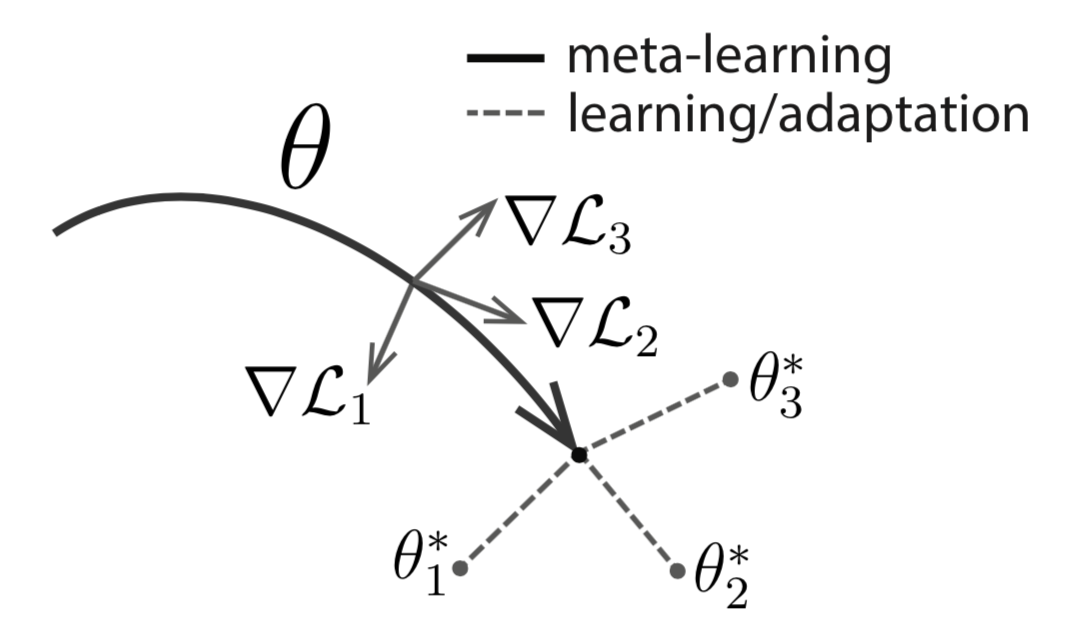
\includegraphics[scale=0.23]{chapters/assets/fsl/maml.png}
    \caption{MAML tries to find optimal generalised weights, by first finding optimal weights in the inner learning phase. Image from \parencite{Finn2017Model-agnosticNetworks}.}
    \label{fig:maml}
\end{wrapfigure}
\textbf{Meta-learning} is most commonly understood as \textquote{learning to learn}, which refers to the process of improving a learning algorithm over multiple learning episodes and was first proposed by \textcite{schmidhuber:1987:srl}. On the contrary, conventional ML improves model predictions on multiple data instances. 
During base learning, an \emph{inner} learning algorithm solves a task such as image classification, defined by a dataset and an objective. During meta-learning, an \emph{outer} algorithm updates the inner learning algorithm so that the model it learns improves an outer objective.
The learning episodes of the base task, namely tuples of the image $\bfitx_i$ and associated label $y_i$, can be seen to provide the instances that the outer algorithm needs to learn the base learning algorithm

MAML is a gradient-based \textbf{meta learning} method. It is a technique that works with any model that learns through gradient descent. It trains a model to find an optimal set of weights that can be quickly adapted to a new task, through a few gradient descent steps. The meta-learner tries to find an initial set of weights that are not only useful for adapting to various problems, but also can be adapted quickly (in a small number of steps) and efficiently (using only a few examples).
\Cref{fig:maml} illustrates how MAML should work at meta-test time. We are looking for a pre-trained parameter that can reach near-optimal parameters for every task in one or a few gradient steps.

This approach is fairly simple and has several advantages. It does not make any assumptions about the form of the model. It is quite efficient - no additional parameters are introduced for meta-learning, and the learner strategy uses a known optimisation process (gradient descent), rather than having to come up with one from scratch. It can also be easily applied to a number of domains, including classification, regression, and reinforcement learning. However, it can be computationally expensive due to the use of higher-order gradients, as we will see.

\subsection{Meta-training}\label{ssec:meta-training}
More formally, we define a \textbf{base model} to be a neural network $\ft$ with meta-parameters $\symbfit \theta$. We want to learn an initial $\symbfit{\theta}^\star = \symbfit{\theta}_0$ that, after a small number $n$ of gradient update steps on data from a support set $\mcS_b$ to obtain $\symbfit{\theta}_n$, the network performs well on the query set of that task $\mcQ_b$. Here, $b$ is the index of a particular task $\mcT_b$. The $n$ gradient update steps form what is known as the \textbf{inner-loop update process}. The updated base-network parameters after $i$ steps on data from the support task $\mcS_b$ can be expressed as
\begin{equation}
\label{eqn:inner-update}
\symbfit{\theta}_{i}^{b}=\symbfit{\theta}_{i-1}^{b}-\eta \nabla_{\symbfit{\theta}} \mathcal{L}_{S_{b}}\left(f_{\symbfit{\theta}_{i-1}^{b}}\right),
\end{equation}
where $\eta$ is the learning rate, $\symbfit{\theta}_i^b$ are the weights of the base network after $i$ steps with task $\mcT_b$, $\mathcal{L}_{S_{b}}\left(f_{\symbfit{\theta}_{i-1}^{b}}\right)$ is the loss on the support set of task $b$ after $(i-1)$ (the previous step) update steps. Assuming that our \textit{task batch} (a batch of tasks instead of images) size is $B$ we can define a meta-objective, which can be expressed as:
\begin{equation}
\label{eqn:meta-obj}
\mathcal{L}_{m e t a}\left(\symbfit{\theta}_{0}\right)=\sum_{b=1}^{B} \mathcal{L}_{\mcQ_{b}}\left(f_{\symbfit{\theta}_{n}^{b}\left(\symbfit{\theta}_{0}\right)}\right),
\end{equation}
where we explicitly show the dependence of $\symbfit{\theta}_n^b$ on $\symbfit{\theta}_0$, given by unrolling \Cref{eqn:inner-update}. The meta-objective in \cref{eqn:meta-obj} measures the quality of an initialisation $\symbfit{\theta}_0$ in terms of the total loss of using that initialisation over a collection of tasks (i.e. a batch of tasks).
This meta objective is now minimised to optimise the initial parameter value $\symbfit{\theta}_0$, this $\symbfit{\theta}_0$ contains within it the across-task experiences and knowledge. This process of optimising for the meta-objective is called the \textbf{outer-loop} update process.
The resulting update process is given by:
\begin{equation}
\label{eqn:meta-update}
\symbfit{\theta}_{0}=\symbfit{\theta}_{0}-\beta \nabla_{\symbfit{\theta}} \sum_{b=1}^{B} \mathcal{L}_{\mcQ_{b}}\left(f_{\symbfit{\theta}_{N}^{b}\left(\symbfit{\theta}_{0}\right)}\right),
\end{equation}
where $\beta$ is a learning rate and $\mathcal{L}_{\mcQ_b}$ denotes the loss on the query set for task $\mcT_b$.
For more details, please refer to \parencite{Finn2017Model-agnosticNetworks, antoniou2018train}.
\section{Prototypical Networks}\label{ssec:protonets}

Prototypical networks are a type of \textbf{metric learning} models. The core idea in metric learning is similar to nearest neighbours algorithms ($k$-NN classifier and $k$-means clustering) and kernel density estimation. The goal of Metric Learning is to learn a representation function that maps objects into an embedded space. The distance in the embedded space should preserve the objects' similarity; similar objects get closer, and dissimilar objects get far away. The similarity metric is learnt by a kernel function $f_{\symbfit{\theta}}$, parameterised by $\symbfit{\theta}$. The distances measured by the kernel function are converted into probabilities on a set of labels $y_i \forall i$ by means of a softmax or sigmoid function. Both $\ccclr$ and $\samptr$ make use of prototypical networks for classification because this method is simple, yet robust, as evidenced by the performance of $\ccclr$ and $\samptr$.

Prototypical networks learn a non-linear function, $f_{\symbfit \theta}$, that maps the input to a feature vector in an embedding space (or representation space) using a parameterised neural network in a supervised manner. The embeddings of the $K$-shots for each of the $N$-classes are averaged to compute the \textbf{class prototypes}. Traditionally, a \textit{prototype} is an entity that is the archetypal form of \textquote{something}, for example, Boeing $777$\footnote{\url{https://www.boeing.com/commercial/777/}} jets are prototypes of modern large passenger jets.
Here, a class prototype $\symbfit{c}_k$ plays a similar role; it is a feature vector that is defined for every class $k \in \mathcal{C}$, as the mean vector of the embedded support set samples in class $k$, and is calculated as:
\begin{equation}
    \symbfit{c}_{k}=\frac{1}{|\mcS_{k}|} \sum_{({\symbfit x}_i, y_i) \in {\mcS_k}} f_{\symbfit \theta}(\symbfit{x}_{i}).
    \label{eqn:fsl-proto-calc}
\end{equation}

\begin{figure}[ht]
    \centering
    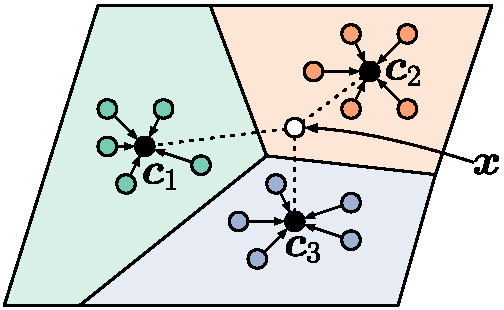
\includegraphics[scale=0.85]{chapters/assets/fsl/prototype_fewshot_v3.pdf}
    \caption{Few-shot prototypes $\symbfit{c}_k$ are computed as the mean of embedded support examples for each class. Image sourced from \parencite{Snell2017PrototypicalLearning}.}
    \label{fig:protonets}
\end{figure}

The distribution over classes for a given query input $\symbfit{x}$ is a softmax over the inverse of the distances between the embedding of the query data and the prototype vectors:
\begin{equation}
    P(y=k\vert\symbfit{x})=\operatorname{softmax}\left(-d(f_\theta(\symbfit{x}), \symbfit{c}_k)\right) = \frac{\exp(-d(f_\theta(\symbfit{x}), \symbfit{c}_k))}{\sum_{k^\prime \in \mathcal{C}}\exp(-d(f_\theta(\symbfit{x}), \symbfit{c}_{k^\prime}))}
    \label{eqn:fsl-proto-classification}
\end{equation}
where $d$ can be any distance function, as long as it is a differentiable operation to allow gradient-based learning. In the original work, \textcite{Snell2017PrototypicalLearning} use the Euclidean distance metric.

Learning is carried out by minimising the negative log likelihood $J(\symbfit{\theta})$ and performing stochastic gradient descent over the same to update the kernel's parameters $\symbfit{\theta}$:
\begin{equation}
    J(\symbfit{\theta})=-\log P_{\symbfit \theta}(y=k \vert \symbfit{x}).
\end{equation}

\subsection{Re-interpretation of the Prototypical Classifier as a Linear Model}\label{ssec:proto-reint-linmodel}

As explained by \textcite{Snell2017PrototypicalLearning}, Prototypical Networks can be re-interpreted as a linear classifier applied to a learned representation $f_{\symbfit{\theta}}(\bfitx)$. Using the Euclidean distance \(d(\symbfit{z}_i, \symbfit{z}_j)=\left\|\symbfit{z}_i-\symbfit{z}_j\right\|^{2}\) in \Cref{eqn:fsl-proto-classification} makes the model equivalent to a linear model and the output logits can be expressed as:
\begin{align}
        -\left\|f_{\symbfit \theta}(\symbfit{x})-\symbfit{c}_{k}\right\|^{2}&=-f_{\symbfit \theta}(\symbfit{x})^{\top} f_{\symbfit \theta}(\symbfit{x})+2 \symbfit{c}_{k}^{\top} f_{\symbfit \theta}(\symbfit{x})-\symbfit{c}_{k}^{\top} \symbfit{c}_{k} \nonumber\\
        2 \symbfit{c}_{k}^{\top} f_{\symbfit \theta}(\symbfit{x})-\symbfit{c}_{k}^{\top} \symbfit{c}_{k}&=\symbfit{W}_{k}^{\top} f_{\symbfit \theta}(\symbfit{x})+b_{k} \text {, where } \symbfit{W}_{k}=2 \symbfit{c}_{k} \text { and } b_{k}=-\symbfit{c}_{k}^{\top} \symbfit{c}_{k}
        \label{eqn:proto-lin-layer}
\end{align}

Based on \Cref{eqn:proto-lin-layer}, we can see that the $k\textsuperscript{th}$ unit of an equivalent linear layer therefore has weights \(\symbfit{W}_k=2\symbfit{c}_k\) and biases $b_k=-\symbfit{c}_{k}^{\top} \symbfit{c}_{k}=-\left\| \symbfit{c}_k \right\|^2$, which are both differentiable with respect to $\symbfit{\theta}$ as they are a function of $f_{\symbfit \theta}$. \textcite{Snell2017PrototypicalLearning} hypothesise that this linear classifier is effective because all the required non-linearity can be learnt within the embedding function $f_{\symbfit \theta}$.

This interpretation also allows us to create a task-specific linear classifier layer for each episode where the layer weights are initialised based on the equivalent weights and biases of the prototypical network as defined above and in \Cref{eqn:proto-lin-layer}. Subsequently, this layer can then be optimised as usual on the given support set. When computing the update for $\symbfit{\theta}$, we allow gradients to flow through the Prototypical Network-equivalent linear layer; we may also \textbf{freeze} the embedding network $f_{\symbfit \theta}$ if we only wish to train the Prototypical Network-equivalent linear layer.


\section{Unsupervised Few-Shot Learning}\label{sec:u-fsl}

So far, we have only discussed few-shot learning in a supervised setting. However, a more challenging scenario is the unsupervised setting. Recall that the dataset in the supervised setting is given as \(\mathcal{D} = \{({\symbfit x}_i, y_i)\}_{i = 1}^{M}\) which implies that we have the true class labels $y_i$ available during training time. In the unsupervised setting, we no longer have access to the true labels during the training period. 

Then a question naturally arises: How do we create valid tasks (see \Cref{sec:formalising-fsl}) if we do not have access to the true labels? This is an important question; consider \Cref{fig:fsl-tasks} where we illustrate (\nwks{3}{2}) shots, we see that each of the $3$ classes has exactly $2$ samples. Tasks like this would be difficult to create without labels. To overcome this, we shall discuss some creative methods in the following sections.

\subsection{CACTUs}\label{ssec:ufsl-cactus}
CACTUs was one of the first methods aimed at solving the unsupervised few-shot learning problem \parencite{Hsu2018UnsupervisedMeta-Learning}. CACTUs uses MAML as part of its training mechanism to obtain a generalisable model. CACTUS also retains the episodic task-based training strategy introduced by MAML \parencite{Finn2017Model-agnosticNetworks}. Unlike MAML, however, a major aspect of CACTUs is dedicated to a clever \textbf{task creation} technique, as it cannot be fed standard tasks, as discussed above.
\begin{figure}[ht]
    \centering
    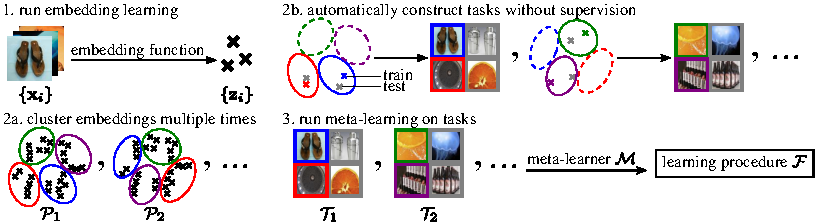
\includegraphics[width=\linewidth]{chapters/assets/fsl/cactus.pdf}
    \caption{Illustration of CACTUs, image from \parencite{Hsu2018UnsupervisedMeta-Learning}. }
    \label{fig:cactus}
\end{figure}
The idea of CACTUs is to use a separate embedding learning algorithm $\mathcal{E}$ on $\bfitx_i \in \mathcal{D}$ to produce embeddings $\{\symbfit{z}_i\}$. It then uses $k$-means clustering on $\{\symbfit{z}_i\}$ $P$ times to generate a set of partitions $\mathcal{P}_P = \{\mathcal{C}_P\}$. CACTUs can technically make use of any self-supervised (more generally, unsupervised) representation learning method to train $\mathcal{E}$. \textcite{Hsu2018UnsupervisedMeta-Learning} choose to use DeepCluster \parencite{caron2018deep}, BiGAN \parencite{berthelot2018understanding}, ACAI \parencite{donahue2016adversarial}, and InfoGAN \parencite{chen2016infogan}. 

CACTUs then samples a partition, $\mathcal{P}$, randomly from the set of partitions $\{\mathcal{P}_P\}$, following which a cluster $\mathcal{C}_n$ is randomly sampled from the partition $\mathcal{P}$. The cluster sampling process is carried out $N$ times for each of the classes desired in a (\nwks{N}{K}) task. Similarly, the process is repeated for $Q$ query images. Finally, the randomly sampled support and query images are used to create a \textbf{synthetic} task that is fed into MAML.

A major concern here is that CACTUs is dependent on bigger models, like AlexNet \parencite{AlexNet2012}, using powerful self-supervised learning methods on a small dataset like \miniImagenet{}. The embeddings (representations) generated by this larger model are then used to create synthetic tasks to train a simpler Conv$4$ architecture. It has been known for quite some time that larger models consistently offer better performance and representations \parencite{Dosovitskiy2020, He2015}, these better representations indirectly aid a smaller Conv$4$ to learn better. The entire premise in the few-shot learning space is to learn a generalisable model quickly. Therefore, by using parameter heavy models and computationally intensive algorithms we defeat the purpose of a self-contained end-to-end few-shot learning algorithm.

\subsection{UMTRA} \label{ssec:umtra}

Unsupervised Meta-learning with Tasks constructed by Random sampling and Augmentation (UMTRA), is another method that uses a MAML style training strategy with inner and outer objectives in an unsupervised fashion.
Unlike CACTUs (\Cref{ssec:ufsl-cactus}), the focus of UMTRA is not on generating ideal tasks. 
Instead, the idea behind UMTRA can be summarised in one line; it is an unsupervised method that uses augmentations of the images in a given episode to create a valid query set. This allows it to generate a \textquote{labelled} query set for the outer objective and can perform well if we span the entire space of the classes.

\begin{figure}[ht]
    \centering
    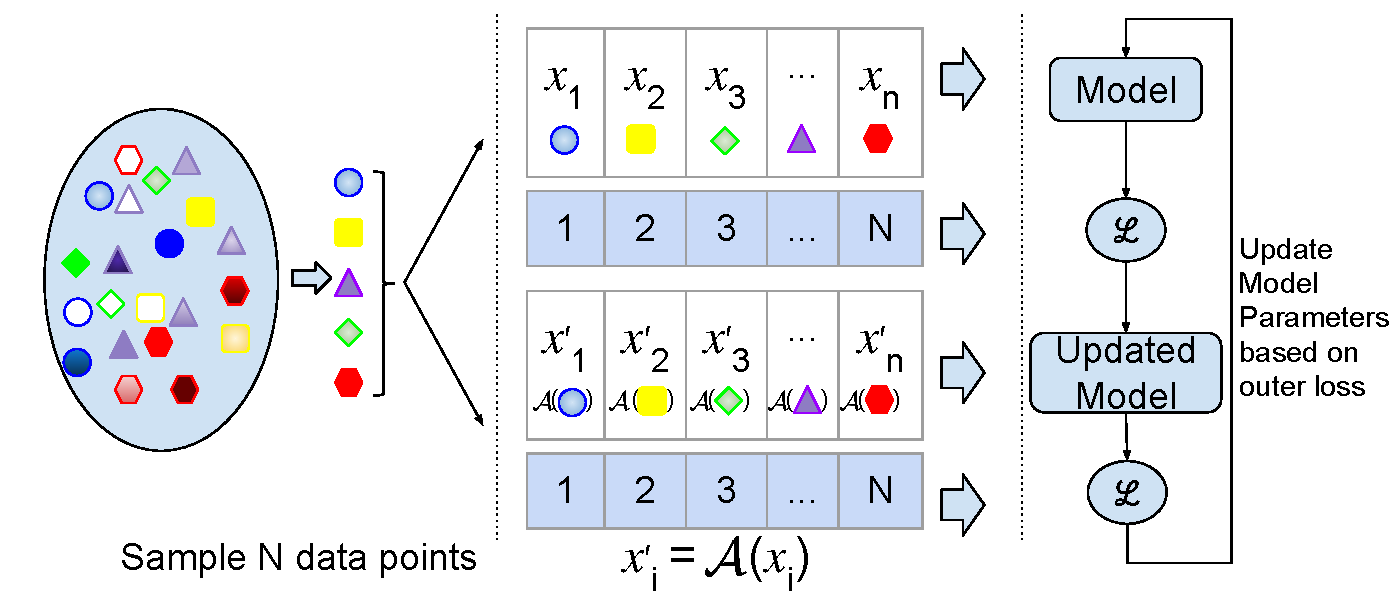
\includegraphics[width=\linewidth]{chapters/assets/fsl/UnsupervisedMetaTraining3.pdf}
    \caption{We start from a dataset of unlabelled data. The training data is created by randomly choosing $N$ samples $\bfitx_i$ from the dataset. The query data is created by applying the augmentation function $\mathcal{A}$ to each sample from the training data. Image borrowed from \parencite{Khodadadeh2018UnsupervisedClassification}.}
    \label{fig:umtra}
\end{figure}

The functioning of UMTRA is illustrated in \Cref{fig:umtra}, where $N$ data points are randomly sampled, each of the $N$ random samples is given its own unique class label. Subsequently, each sample $\symbfit{x}_i$ is augmented using an augmentation function $\mathcal{A}$ that gives an augmented image $\symbfit{x}_i^\prime$. 
The reason this works is that each augmented image will share its class label with the original image. Therefore, the outer objective will always have samples of the same class available for it to learn from. 

\subsection{ProtoTransfer}\label{ssec:prototransfer}

Until now, we have discussed \nameref{ssec:ufsl-cactus} and \nameref{ssec:umtra}, both of which use \nameref{sec:maml} and episodic training to solve the few-shot classification problem.
However, several recent studies have questioned the necessity of meta-learning for few-shot classification \parencite{goodemballneed2020, Medina2020Self-SupervisedClassification, dhillon2019baseline, ziko2020laplacian, boudiaf2020information,chen2021self}.
They report competitive performance on few-shot benchmarks without episodic training or few-shot task-based experiences during training. 
These methods follow an approach where they aim to solve the few-shot learning problem using transfer-learning. First, they pre-train a feature-extractor and then fine-tune a simple classification layer (usually a linear layer) with standard cross-entropy loss.
In fact, both our methods (\ccclr{} and \samptr{}) are based on this paradigm and comfortably outperform unsupervised/supervised MAML based methods.

Some of these methods \parencite{Medina2020Self-SupervisedClassification, goodemballneed2020, das2022confess} in the space demonstrate that the transfer learning approach outperforms meta-learning based methods in standard in-domain and cross-domain settings, where the training and novel classes come from totally different distributions.
%
\begin{figure}[ht]
\centering
\begin{minipage}{\textwidth}
  \centering
  \setlength{\unitlength}{1cm}
  
    \begin{picture}(13.5,5)
    \put(0,0){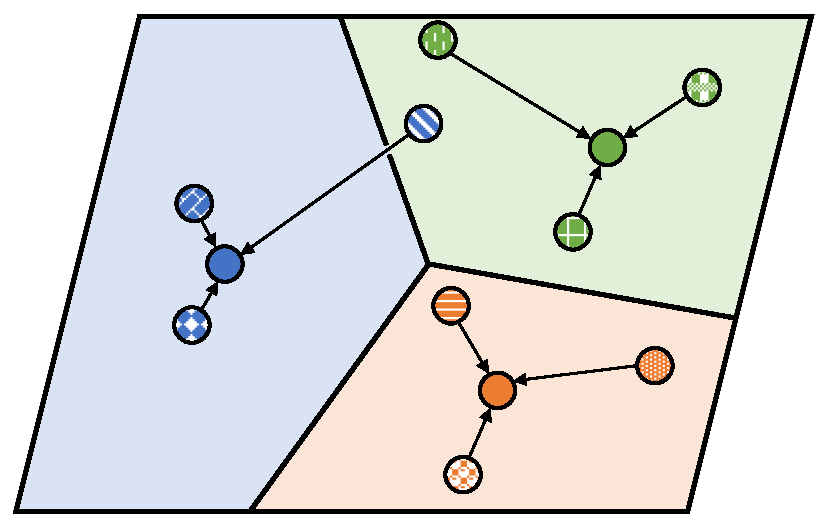
\includegraphics[scale=0.45]{chapters/assets/fsl/selfsupproto.pdf}}
    
    \put(7.3,0){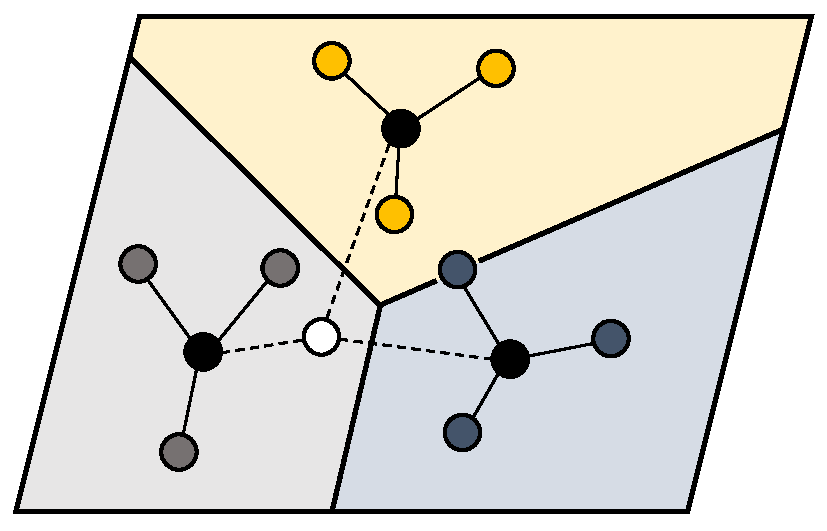
\includegraphics[scale=0.45]{chapters/assets/fsl/protofinetune.pdf}}
    \put(1.9,1.9){$\scriptstyle f_\theta(\symbfit{x}_i)$}
    \put(1,1.2){$\scriptstyle f_\theta(\tilde{\symbfit{x}}_{i,1})$}
    \put(1,2.8){$\scriptstyle f_\theta(\tilde{\symbfit{x}}_{i,2})$}
    \put(3.1,2.7){$\scriptstyle f_\theta(\tilde{\symbfit{x}}_{i,3})$}
    
    \put(4.8,2.8){$\scriptstyle f_\theta(\symbfit{x}_{2})$}
    
    \put(3.9,.8){$\scriptstyle f_\theta(\symbfit{x}_{1})$}

    \put(10.5,2.9){$\scriptstyle \symbfit{c}_{1}$}
    \put(8.4,1.1){$\scriptstyle \symbfit{c}_{2}$}
    \put(11.3,1.1){$\scriptstyle \symbfit{c}_{3}$}
    
    \put(9.3,1.1){$\scriptstyle f_\theta(\symbfit{q})$}
    \end{picture}\\
    \hspace{-.2cm}(a) Self-Supervised Prototypical Pre-Training \hspace{.8cm} (b) Prototypical Fine-Tuning \& Inference
  
  \label{fig:sub2}
\end{minipage}
\caption{Self-Supervised Prototypical Transfer Learning. (a): In the embedding, original images $\symbfit{x}_i$ serve as class prototypes around which their $Q$ augmented views $\tilde{\symbfit{x}}_{i,q}$ should cluster. (b): Prototypes $\symbfit{c}_{k}$ are the means of embedded support examples for each class $n$ and initialise a final linear layer for fine-tuning.
An embedded query point $\symbfit{q}$ is classified via a softmax over the fine-tuned linear layer.
Image sourced from \parencite{Snell2017PrototypicalLearning}.}
\label{fig:prototransfer}
\end{figure}

One such method that we shall focus on is ProtoTransfer \parencite{Medina2020Self-SupervisedClassification}. Unlike \nameref{ssec:ufsl-cactus} and \nameref{ssec:umtra} ProtoTransfer does not rely on a task-based episodic training regime and does not use MAML for its training. 
Instead, ProtoTransfer uses a form of \hyperref[sec:contrastive-learning]{contrastive representation learning} that is similar to and inspired by \nameref{ssec:simclr}. 
ProtoTransfer consists of two phases: (i) \textbf{pre-training} on a large dataset of \textquote{base} classes. This is followed by (ii) \textbf{fine-tuning} on an unseen dataset consisting of \textquote{novel} classes. 

\textcite{Medina2020Self-SupervisedClassification} call their pre-training method \textbf{ProtoCLR}, and in principle it is extremely similar to \nameref{ssec:simclr}.
ProtoCLR uses the original image, $\bfitx_i$, and $Q$ augmentations, $\{\Tilde{\bfitx}_{i,q}\}_{q=1}^Q$. In order to learn the metric embedding function, $f_{\symbfit{\theta}}(\cdot)$, a contrastive loss is used here to ensure that all $Q$ augmentations have the same representation as the original image. 
\nameref{ssec:simclr} on the other hand, uses two augmentations of the same image and ensures similarity between them by means of a contrastive loss. Although not the same, one can see that ProtoCLR is very inspired by methods such as \nameref{ssec:simclr}.

\begin{tcolorbox}[title=Link between self-supervision and an episode]
Consider a mini-batch that contains $n$ random samples $\{{\bfitx_i}\}_{i=1 \ldots n}$ from the training set $\mathcal{D}^\textup{tr}$.
As our self-supervised setting does not assume any knowledge about the base class labels $\symbfit{y} \in \mathcal{D}^\textup{tr}$, we treat each sample as its own class. Thus, each sample $\bfitx_i$ serves as a $1$-shot support sample and class prototype. For every prototype $\bfitx_i$, $Q$ randomly augmented samples $\Tilde{\bfitx}_{i,q}$ are used as query samples.
\end{tcolorbox}

Following the ProtoCLR pretraining phase, we have a fine-tuning phase called \textbf{ProtoTune} and it is a supervised phase. In the fine-tuning phase, the learnt embedding $f_{\symbfit{\theta}}(\cdot)$ is used to address the \textbf{target problem} of few-shot image classification, where we are presented with test tasks episodically, each with their own support and query.
ProtoTune is based on the linear layer interpretation of the Prototypical classifier (see \Cref{ssec:proto-reint-linmodel}). It uses each task's support set to initialise the linear classifier and fine-tune it on subsets of the support set for some iterations, randomly sampling different subsets of support images in each iteration.

ProtoTransfer was chosen as the base for \ccclr{} and \samptr{} due to its robustness and simplicity of self-supervision. Although both \ccclr{} and \samptr{} are inspired by ProtoTransfer, the similarities only extend to their shared self-supervised nature and in the case of \samptr{} there is a reimagined network and fine-tuning phase based on \hyperref[chap:optimal-transport]{optimal transport} that has the potential to be useful even outside of few-shot learning.